\documentclass[AMA,twocolumn]{USG} %twocolumn
\usepackage{anyfontsize} %
\usepackage{parskip}     % gap between paragraphs, no first-line indent
\setlength{\parskip}{0.5\baselineskip}
\usepackage{colortbl}   % For coloring table lines
\usepackage{xcolor}     % For color definitions
\usepackage{lipsum}
\usepackage{cleveref}
\usepackage{siunitx}
\graphicspath{{./images/}}
\articletype{ORIGINAL ARTICLE}%
\received{20 January 2023}
\revised{21 January 2023}
\accepted{22 January 2023}
\journal{Earthquake Engineering \& Structural Dynamics}
\volume{0}
\copyyear{2024}
\startpage{1}
\articledoi{10.1002/0000}
%\raggedbottom

%%
%\renewcommand\ShowFrameLinethickness{0.15pt}
%\renewcommand*\ShowFrameColor{\color{red}}


\begin{document}
\title{Discontinuum modelling of the quasi-static and seismic response of a Dutch calcium silicate masonry building with modular steel-frame retrofit}
%\subtitle{Subtitle}
\transtitle{Seismic discontinuum analysis of a retrofitted masonry building}
\author[1,2]{Yopi Prabowo Oktiovan}
\author[3,4]{Nicol\`{o} Damiani}
\author[1]{Amirhossein Ghezelbash}
\author[1]{Francesco Messali}

\authormark{OKTIOVAN \textsc{et al.}}
\titlemark{PLEASE INSERT YOUR ARTICLE TITLE HERE}

\address[1]{Faculty of Civil Engineering and Geosciences, \orgname{Delft University of Technology}, Stevinweg 1, 2628 CN Delft, \country{The Netherlands}}
\address[2]{Research Centre Built Environment, Structural Safety and Earthquakes, \orgname{Hanze University of Applied Sciences}, Groningen, \country{The Netherlands}}
\address[3]{Department of Civil Engineering and Architecture, \orgname{University of Pavia}, via Ferrata 3, 27100 Pavia, \country{Italy}}
\address[4]{\orgname{European Centre for Training and Research in Earthquake Engineering (EUCENTRE)}, via Ferrata 1, 27100 Pavia, \country{Italy}}
 
\corres{Yopi Prabowo Oktiovan. \email{y.p.oktiovan@tudelft.nl}}

\presentaddress{Zernikeplein 7, 9747 AS Groningen}

% \fundingInfo{National Key Research and Development Program of China, Grant/Award Number: 2021YFB1715500; National Natural Science Foundation of
% China, Grant/Award Number: 12072071; Scientific Research Foundation of Hunan Provincial Education Department, Grant/Award Number: 22A0104;
% Fundamental Research Funds for the Central Universities, Grant/Award Number: N2225027.}

\keywords{distinct element method | calcium silicate masonry | induced seismicity | seismic retrofit | incremental dynamic analysis | modular steel-frame exoskeleton}

\transkeywords{DEM | calcium silicate masonry | induced seismicity | seismic retrofit | incremental dynamic analysis | modular steel-frame exoskeleton}

\abstract[ABSTRACT]{Induced seismicity from gas extraction in the Groningen field has exposed a large stock of Dutch unreinforced masonry (URM) buildings to seismic demands they were not designed to resist. 
Calcium silicate (CS) terraced houses represent the dominant affected typology, with joint-controlled failure kinematics that motivate a discontinuum modelling approach. 
This paper investigates the quasi-static and dynamic performance of a representative Dutch CS terraced house through three-dimensional discontinuum analysis using the Masonry Advanced Softening cONtact (MASON) model, combining tension cut-off, cohesion-softening friction, and compression-cap failure at mortar interfaces. 
The model is validated against a full-scale quasi-static cyclic pushover test at TU Delft, reproducing the peak base shear, cumulative energy dissipation, and coupled in-plane and out-of-plane damage pattern. 
The framework is then applied in incremental dynamic analysis with a Groningen-specific ground motion record (EQ-NPR) to identify the unreinforced near-collapse limit, using interstorey drift ratio against PGA bounded by code- and empirically based thresholds. 
Collapse is driven by in-plane pier splitting that degrades transverse-wall corner restraint. 
The framework is extended on an exploratory basis to the same typology retrofitted with the Resisto 5.9 modular steel-frame exoskeleton. 
Component-level validation against EUCENTRE cyclic pier tests precedes building-scale application to calibrate the retrofit parameters. 
A near-collapse intensity gain factor of approximately 1.7 is obtained, with peak in-plane displacements reduced by roughly 75\% at matched intensity. 
Together, the dynamic and retrofit assessments show that the framework can identify the governing collapse mechanism and the limiting component of a retrofit system, offering a basis for targeted experimental campaigns.}

\abbr{5-FU, 5-fluorouracil; CFD, computational fluid dynamics; CH, channel; EFS, event-free survival; GBM, glioblastoma multiforme; OS, overall survival; PFS, progression-free
survival; SD, standard deviation.}

\contributed{Hao Zhang and Pengyue D. Guo contributed equally to this study.}

% \dedicated{Dedicated to Srivivasa Ramanujano on the occasion of his 125th birth anniversary.}

\copyright{This is an open access article under the terms of the \href{Creative Commons Attribution-NonCommercial}{Creative Commons Attribution-NonCommercial} License, which permits use, distribution and reproduction in any medium, provided the
original~work~is~properly cited and is not used for commercial purposes.
\\[5pt]
  ©  2024 The Author(s) \textit{AIChE Journal} published by Wiley Periodicals LLC on behalf of American Institute of Chemical Engineers.}

%\openaccessstatement

\maketitle
%\afterpage{\aftergroup\restoregeometry}

%\onecolumn

\section{Introduction}\label{sec:Intro}
\lipsum[1-3]
%==============================================================================
\section{Experimental description}\label{sec:experiment}
The building-scale benchmark is a quasi-static cyclic pushover test, complemented by dynamic identification, performed on a full-scale two-storey assemblage at TU Delft~\cite{Ravenshorst2016StructuralTest}.
The specimen, designated TUD-BUILD-1, reproduced the inner load-bearing leaf of a calcium silicate (CS) terraced house, typical of Dutch residential construction of the 1970s--1980s.
Houses of this typology have cavity walls, a structural CS inner leaf that carries the loads, and a non-structural clay-brick veneer joined to it by thin ties that transfer negligible in-plane shear. 
The veneer is disregarded in the seismic assessment, and the TUD-BUILD-1 specimen reproduces only the inner structural leaf. 
Conceived as a model-validation benchmark, its defining feature is a pair of slender piers that govern the response in the loading direction (\Cref{fig:exp_geometry}).

\begin{figure*}[!ht]
    \centering
    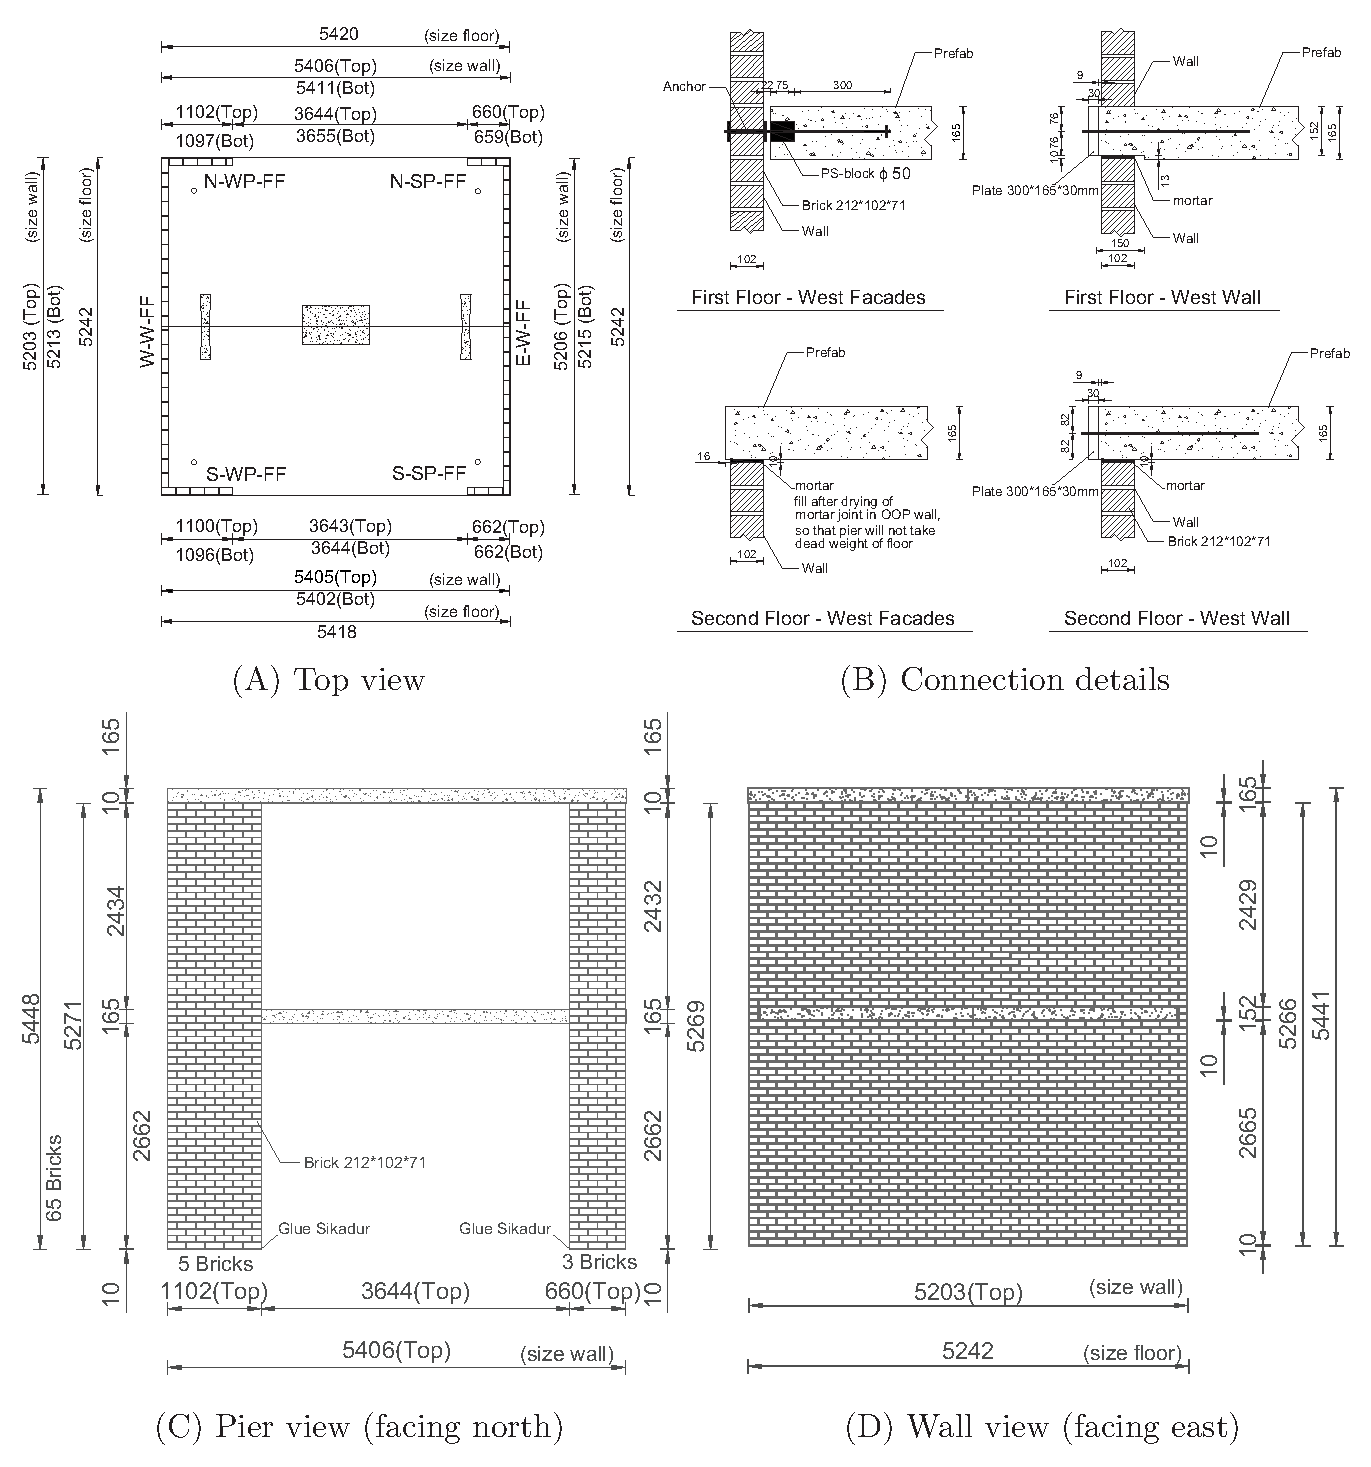
\includegraphics[width=.8\linewidth]{Figures/EXP_Details.eps}
    \caption{Geometry and construction details of TUD-BUILD-1~\cite{Ravenshorst2016StructuralTest}: (A) plan with wall nomenclature; (B) floor-to-wall connections (first floor anchored, second floor bearing only); (C) north pier with the wide and narrow piers; (D) east load-bearing wall. Dimensions in mm.}
    \label{fig:exp_geometry}
\end{figure*}

\subsection{Geometry and materials}
The assemblage comprises two longitudinal load-bearing walls on the west and east sides and two pier walls on the north and south sides, each pier wall formed by a wide (\qty{1100}{\milli\meter}) and a narrow (\qty{660}{\milli\meter}) pier (\Cref{fig:exp_geometry}A).
The masonry was laid in stretcher bond from CS bricks of nominal size \qtyproduct[product-units=single]{210x71x102}{\milli\meter} with \qty{10}{\milli\meter} mortar joints. 
The corner connection between piers and longitudinal walls was toothed.
The two floors each consist of two prefabricated reinforced-concrete slabs (\qty{165}{\milli\meter} thick, class C53/65) joined in-situ by wet mortar joints.
The structure was built on a steel substructure, with the first masonry course glued to the base so that cracking in the base would initiate at the first bed joint rather than at the steel interface.
The material properties used for the numerical calibration are summarised in \Cref{sec:model} and were characterised in the companion material campaign~\cite{Jafari2022AStructures,Jafari2021MaterialAnalysis}.

\subsection{Floor-to-wall connections}
Both floors span between and rest on the west and east load-bearing walls, and they differ in how they connect to the north and south piers (\Cref{fig:exp_geometry}B). 
At the first floor, the slab is tied horizontally to the piers by \qty{6}{\milli\meter} cast-in anchors (three in each narrow pier and five in each wide pier), forming a positive in-plane connection between diaphragm and piers. 
At the second floor, the pier-to-slab joint was mortar-filled only after the slab had been placed, so that the piers carry no floor dead load.
The second-floor slab is therefore only weakly tied to the piers. 
The limited restraint afforded by this second-floor connection is revisited in interpreting the building response.

\subsection{Test set-up and loading protocol}
Lateral load was applied through four actuators, two per floor, reacting against a braced steel tower.
Displacement control was imposed at the second-floor jacks, with a 1:1 force ratio enforced between the second and first floors through coupled actuator forces, and the rigid RC diaphragms redistributed the load to the walls.
Specimen displacements were measured absolutely relative to an independent, stiff wooden frame, with string potentiometers on the in-plane side and laser displacement sensors on the out-of-plane side.
The protocol comprised three phases of increasing amplitude, with three runs applied at each target. 
The initial phase (cycles 1--8) reached a second-floor amplitude of about \qty{3}{\milli\meter}, the pre-peak phase (cycles 9--14) about \qty{15.5}{\milli\meter}, and the post-peak phase (cycles 15--21) about \qty{82}{\milli\meter}, after which a final half-run to about \qty{92}{\milli\meter} was applied before the test was stopped for safety. 
The second-floor target displacement is reported as the average of the north and south loading points.

Dynamic identification was carried out at three damage stages by disconnecting the actuators and applying hammer impacts. 
The first global mode in the loading (east--west) direction fell from \qty{4.05}{\hertz} to \qty{3.74}{\hertz} and then to \qty{2.5}{\hertz} across the three stages, consistent with the progressive stiffness degradation observed in the pushover response.

\subsection{Observed damage}
Visual inspection after each cycle traced a consistent crack sequence across the three loading phases, summarised on the final pattern of \Cref{fig:exp_crack}.
In the initial phase (up to the second floor displacement, $d_2$, of $\approx$ \qty{3}{\milli\meter}) the response was essentially linear-elastic, and the first cracks were horizontal, opening along the bed joints at the floor-to-wall conections and at the top and bottom of the southern piers (P1 and P2 on the west and east walls, respectively).
These early cracks were detectable only by instrumentation as the crack widths were relatively small.
In the pre-peak phase, the horizontal pier-base cracks became visible, appearing first at the foot of pier P1 ($d_2 \approx \pm 3.2$~mm) and, by $d_2 \approx \pm 9$~mm, at all four piers, while the first diagonal stepped cracks formed in the load-bearing west and east walls.

\begin{figure*}[!ht]
    \centering
    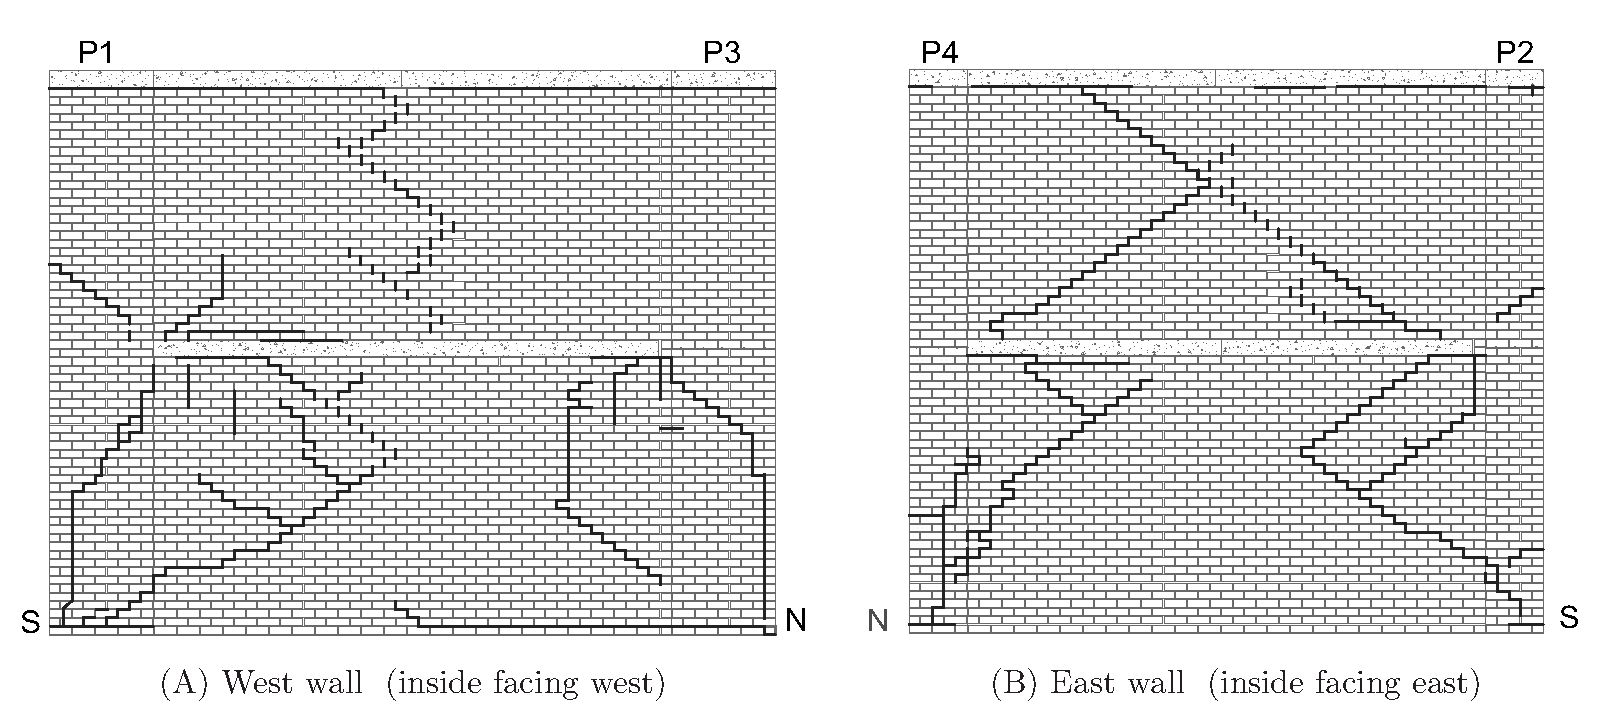
\includegraphics[width=.85\textwidth]{Figures/EXP_Crack.eps}
    \caption{Final crack pattern at the end of the test~\cite{Ravenshorst2016StructuralTest} (inside views): (A) west wall between piers P1 (south) and P3 (north); (B) east wall between piers P4 (north) and P2 (south).}
    \label{fig:exp_crack}
\end{figure*}

In the post-peak phase, the most severe damage occurred in the ground-floor piers, with diagonal and vertical splitting.
Pier P3 cracked and split first ($d_2 \approx \pm 38$~mm), followed by pier P1 ($d_2 \approx \pm 50$~mm), with damage in P3 severe enough that part of it was removed for safety late in the test.
Meanwhile, the load-bearing walls developed the diagonal stepped field shown in \Cref{fig:exp_crack}, along with out-of-plane yield-line cracking, while the unequal pier lengths produced a markedly asymmetric response between the two loading directions.
The final pattern is dominated by in-plane shear following the bed and head joints, with local vertical splitting through the brick units on the west piers.
Damage spread across both the piers and the load-bearing walls, highlighting that they acted as a coupled system in resisting the in-plane demand.

%==============================================================================
\section{Numerical modelling setup}\label{sec:model}

The TUD-BUILD-1 specimen is reproduced using the three-dimensional distinct element method, which matches the joint-controlled behaviour observed in the test by allowing damage to localise at the mortar interfaces.
This section sets out the discretisation and the MASON contact model governing the unit-mortar interface behaviour, the half-symmetry building model with boundary and connection idealisations, the calibrated material parameters, and the loading and solution scheme adopted for the quasi-static and dynamic analyses.

\subsection{Discretisation and the MASON contact model}
\begin{figure*}[!hb]
    \centering
    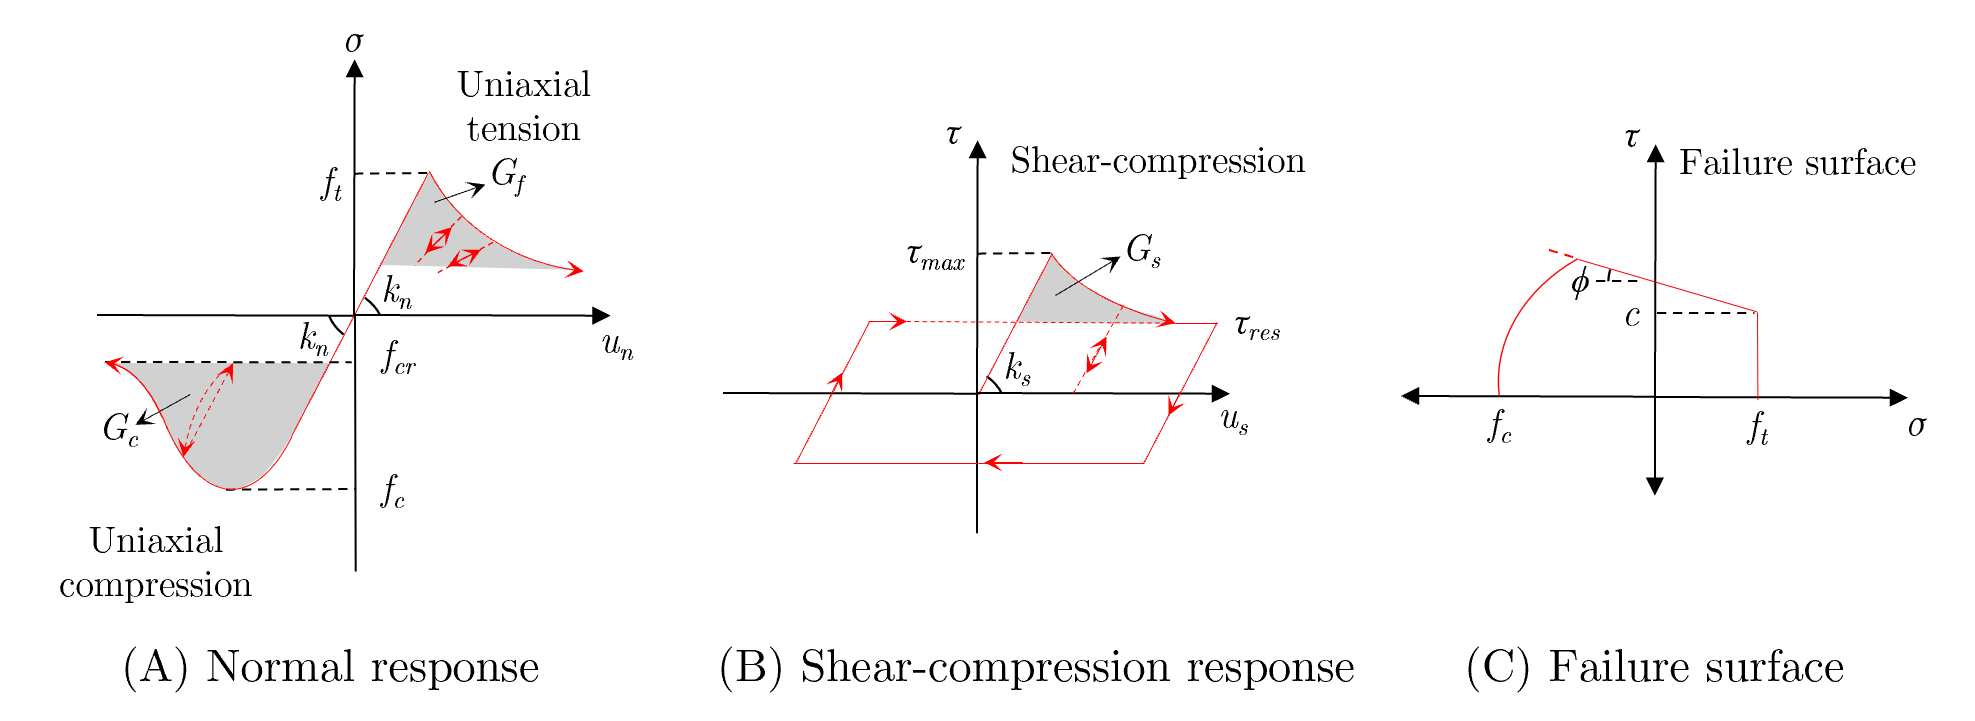
\includegraphics[width=.9\textwidth]{Figures/MASON_NEW_horizontal.png}
    \caption{The MASON contact model~\cite{Oktiovan2026CyclicMethod}: (A) normal response with tension cut-off and compression cap; (B) shear-compression response with cohesion softening; (C) shear--normal failure surface.}
    \label{fig:mason}
\end{figure*}

The assemblage is modelled in three dimensions using the distinct element method, in which the masonry is represented as an assembly of blocks with expanded dimensions that interact through zero-thickness interfaces representing the mortar joints.
Each interface is discretised into triangular sub-contacts, and the contact constitutive model is evaluated at the resulting contact points.
Blocks are treated as rigid in the quasi-static analyses and as deformable in the dynamic analyses (\Cref{sec:dynamic}). 
The rigid idealisation is justified when the nonlinearity concentrates at the interfaces, where rigid blocks reproduce the mechanism at a fraction of the cost of deformable blocks. 
Deformable blocks, meshed internally with elastic modulus $E_b$, are adopted for the dynamic analyses because the steel-frame retrofit is represented by beam finite elements that couple only to the nodal points of deformable meshes and cannot be accommodated by rigid blocks. 
The unreinforced configuration is therefore also run with deformable blocks under dynamic loading, so the unreinforced and retrofitted cases share a single modelling basis, and any difference in response reflects the retrofit rather than the block idealisation.

The interface behaviour follows the Masonry Advanced Softening cONtact (MASON) model~\cite{Oktiovan2026CyclicMethod}, a contact constitutive law that combines three failure mechanisms at the mortar joints (\Cref{fig:mason}).
A tension cut-off governs mode-I opening, with the tensile strength $f_t$ softening to zero over the mode-I fracture energy $G_{f_t}$.
A Coulomb friction law governs mode-II sliding, with the cohesion $c$ softening to a residual value $c_{\mathrm{res}}$ over the mode-II fracture energy $G_{f_s}$ at constant friction angle $\phi$.
A compression cap limits the normal stress and is defined by the compressive strength $f_c$, the compressive fracture energy $G_c$, the cap shape parameters $C_n$, $C_{nn}$ and $C_{ss}$, and the peak $n$.
Unit splitting, seen in the experiment as vertical cracking through the bricks, is reproduced through a potential crack plane at the mid-length of each unit, to which the unit strengths $f_{t,b}$, $c_b$ and $\phi_b$ are assigned.

\subsection{Building model and boundary conditions}
A half-symmetry model is adopted in this study, as presented in \Cref{fig:num_model}.
The rear plane is restrained in the $Y$ direction, which halves the model size and suppresses any torsional and anti-symmetric response.
The simplification is justified by the symmetric plan of the specimen, the uniaxial input applied along the global $X$ direction, and the absence of mass eccentricity.
The masonry is supported on a steel base

\begin{figure}[!ht]
    \centering
    \includegraphics[width=0.85\linewidth]{Figures/TUD_BUILD_NUM_setup.eps}
    \caption{Half-symmetry DEM model of TUD-BUILD-1 and the quasi-static loading scheme.}
    \label{fig:num_model}
\end{figure}
%==============================================================================
\section{Quasi-static analysis of the building}\label{sec:quasistatic}
\lipsum[1-3]
%==============================================================================
\section{Resisto 5.9 retrofit solution and numerical implementation}\label{sec:retrofit-concept}
\lipsum[1-3]
%==============================================================================
\section{Component-level validation of the retrofitted pier}\label{sec:component}
\lipsum[1-3]
%==============================================================================
\section{Incremental dynamic analysis results}\label{sec:dynamic}
\lipsum[1-3]
%==============================================================================
\section{Conclusions}\label{sec:conclusions}
\lipsum[1-3]
A three-dimensional DEM investigation of the quasi-static and dynamic performance of a Dutch calcium silicate terraced house has been presented in unreinforced and Resisto 5.9 retrofitted configurations. The MASON contact constitutive model was validated at component level against the quasi-static cyclic tests of the S-HEA-U and S-HEA-R specimens conducted at EUCENTRE, and at building level against the cyclic pushover test of the TUD-BUILD-1 specimen at TU Delft. The validated framework was applied to a sequential incremental dynamic analysis using the EQ-NPR ground motion record scaled between 20\% and 300\% of the reference amplitude. The main findings are as follows.
 
The building-scale quasi-static validation reproduces the peak base shear within 2\%, the initial stiffness within 25\% for the rigid-block configuration, the cumulative dissipated energy trend up to the middle of the pre-peak phase, and the coupled in-plane and out-of-plane damage mechanism observed in the experiment. The rigid-block and deformable-block configurations yield a comparable peak capacity and a similar failure mechanism, which justifies the transition to deformable blocks in the dynamic analyses without introducing a significant bias.
 
The dynamic analysis of the unreinforced configuration identifies the near-collapse limit at PGA $= 0.41$ g (125\% scale factor of EQ-NPR), based on the convergence of three independent indicators. The ground-storey in-plane IDR exceeds the EC8-3 (2023) threshold and the Messali (2018) characteristic lower bound in both facade piers, and the deformed configuration shows a fully developed diagonal crack band with block separation and corner detachments. The collapse is governed by in-plane rocking and splitting of the ground-floor piers, followed by the out-of-plane overturning of the transverse walls through corner restraint loss.
 
The Resisto 5.9 retrofit extends the near-collapse capacity to PGA $= 0.70$ g (225\% scale factor), a gain factor of 1.7 in ground motion intensity. At matched intensity levels, the retrofit reduces peak in-plane displacements by approximately 75\% and increases the peak base shear by approximately 50\%. The spatial distribution of displacement demand is preserved, so that the retrofit scales the response down proportionally without altering the building deformation shape. The governing collapse mechanism of the retrofitted configuration is a mixed IP-OOP mechanism, in which the steel frames delay but do not prevent pier rocking and toe-crushing. The resulting slab uplift progressively degrades the floor-to-wall mortar joints until the second-floor diaphragm loses its bearing on the transverse walls, which then overturn as near-rigid panels. The floor-to-wall connection is identified as the weakest link of the retrofit system and requires experimental validation.
 
The present study is based on a single ground motion record, a single building typology, and entirely on numerical simulations. The retrofit performance reported here has not been verified experimentally at the building scale, and the findings are conditional on the modelling assumptions adopted for the floor-to-wall and 3D corner connections, whose properties follow the manufacturer design intent rather than measured force-displacement data. Three extensions are identified. A multi-record IDA campaign would quantify the record-to-record variability in the near-collapse identification. A sensitivity analysis on the damping formulation and on the floor-to-wall connection parameters would quantify the epistemic uncertainty in the retrofit performance assessment. Experimental characterisation of the retrofit-to-RC connection detail and of the 3D corner links on CS masonry with precast RC floors would replace the current assumed values and strengthen the quantitative conclusions on the retrofitted near-collapse capacity.

%==============================================================================
\bmsection*{Acknowledgments}
The authors acknowledge the support of the Nederlandse Aardolie Maatschappij (NAM) and Delft University of Technology. The collaboration with the University of Pavia and EUCENTRE on the Resisto 5.9 modelling is gratefully acknowledged.
 
\bmsection*{Financial disclosure}
None reported.
 
\bmsection*{Conflict of interest}
The authors declare no potential conflict of interest.
 
\bmsection*{Data availability statement}
The numerical models and post-processing scripts that support the findings of this study are available from the corresponding author upon reasonable request.
\bibliography{Mendeley}


\end{document}
